\documentclass[border=4pt,12pt]{standalone}
% House style for redrawn exam diagrams (diagram-v4: 0.4pt lines, filled -latex arrows, fine dashes; stipple and hatching drawn as real dots/lines (no PDF/SVG patterns, so they render in every browser and at any scale); transparent background). Every figure \input's this.
\usepackage{amsmath,amssymb}
\usepackage{txfonts}
\usepackage{pdfrender,xcolor}
% \halo{text}: label on shading. The shading stops just around each letter's outline (a thin knock-out that follows the
% glyphs, like the papers' typesetting), never a box. Owner: "I don't want a box around the text".
\newcommand{\halo}[1]{\leavevmode\rlap{\pdfrender{TextRenderingMode=2,LineWidth=2.2pt,LineJoinStyle=1,StrokeColor=white,FillColor=white}#1}#1}
\usepackage{tikz,pgfplots}
\pgfplotsset{compat=1.18}
\usetikzlibrary{arrows.meta,calc,angles,quotes,patterns,patterns.meta,intersections,positioning,decorations.markings,shapes.geometric}
% Stipple and hatching are drawn as actual dots / lines clipped to the region (path picture), NOT as pattern fills:
% SVG <pattern> fills vanish or blur when browsers scale the image, so the owner could not see the shading.
% Each dot is a 0.72pt square (keeps SVGs small; reads as a dot at print size). Dots sit on one global staggered grid, so neighbouring regions line up.
\makeatletter
\newdimen\ex@x \newdimen\ex@y \newdimen\ex@xa \newdimen\ex@ya \newdimen\ex@xb \newdimen\ex@yb \newcount\ex@row
\def\exam@stipplecolor{black!75}\def\exam@dotr{0.42pt}\def\exam@dotgap{2.5}
\def\ex@rowdots{\ifdim\ex@x<\ex@xb \pgfpathrectangle{\pgfqpoint{\dimexpr\ex@x-0.36pt\relax}{\dimexpr\ex@y-0.36pt\relax}}{\pgfqpoint{0.72pt}{0.72pt}}\advance\ex@x by \exam@dotgap pt\relax\expandafter\ex@rowdots\fi}
\def\exam@stipple{%
  \pgftransformreset% dots are sized in real points even inside scaled pictures
  \pgfpointanchor{path picture bounding box}{south west}\ex@xa=\pgf@x \ex@ya=\pgf@y
  \pgfpointanchor{path picture bounding box}{north east}\ex@xb=\pgf@x \ex@yb=\pgf@y
  \pgfsetfillcolor{\exam@stipplecolor}\pgfmathsetmacro\ex@h{\exam@dotgap/2}%
  \pgfmathtruncatemacro\ex@r{floor(\ex@ya/\ex@h)-1}\ex@row=\ex@r\relax
  \ex@y=\ex@r\dimexpr\ex@h pt\relax
  \loop\ifdim\ex@y<\ex@yb
    \pgfmathtruncatemacro\ex@c{floor(\ex@xa/\exam@dotgap)-1}\ex@x=\ex@c\dimexpr\exam@dotgap pt\relax
    \ifodd\ex@row \advance\ex@x by \ex@h pt\fi
    \ex@rowdots
    \advance\ex@y by \ex@h pt \advance\ex@row by 1
    \ifnum\numexpr\ex@row-(\ex@row/4)*4\relax=0 \pgfusepath{fill}\fi% flush every 4 rows: bounded TeX memory, few clip copies in the SVG
  \repeat\pgfusepath{fill}}
\newdimen\ex@d
\def\exam@hatch#1{% #1 = 1 for /, -1 for \ ; lines 45 degrees, 3pt apart
  \pgftransformreset
  \pgfpointanchor{path picture bounding box}{south west}\ex@xa=\pgf@x \ex@ya=\pgf@y
  \pgfpointanchor{path picture bounding box}{north east}\ex@xb=\pgf@x \ex@yb=\pgf@y
  \ex@d=\dimexpr\ex@yb-\ex@ya\relax \ex@x=\dimexpr\ex@xa-\ex@d\relax
  \loop\ifdim\ex@x<\ex@xb
    \ifnum#1>0 \pgfpathmoveto{\pgfqpoint{\ex@x}{\ex@ya}}\pgfpathlineto{\pgfqpoint{\dimexpr\ex@x+\ex@d\relax}{\ex@yb}}%
    \else \pgfpathmoveto{\pgfqpoint{\ex@x}{\ex@yb}}\pgfpathlineto{\pgfqpoint{\dimexpr\ex@x+\ex@d\relax}{\ex@ya}}\fi
    \advance\ex@x by 4.24pt
  \repeat
  \pgfsetlinewidth{0.4pt}\pgfsetstrokecolor{black}\pgfusepath{stroke}}
\def\examstipple{\exam@stipple}\def\examhatch{\exam@hatch}\def\examsetstipplecolor#1{\def\exam@stipplecolor{#1}}\def\examsetdotgap#1{\def\exam@dotgap{#1}}
\makeatother
% (legacy pattern kept for old files)
% staggered stipple like the NESA papers' dotted shading
\pgfdeclarepatternformonly{exam stipple}{\pgfpointorigin}{\pgfqpoint{2.2pt}{2.2pt}}{\pgfqpoint{2.2pt}{2.2pt}}{%
  \pgfpathcircle{\pgfqpoint{0.55pt}{0.55pt}}{0.42pt}\pgfpathcircle{\pgfqpoint{1.65pt}{1.65pt}}{0.42pt}\pgfusepath{fill}}
\tikzset{
  every picture/.style={line width=0.6pt, >={Latex[length=2mm,width=1.3mm]}},
  curve/.style={line width=0.6pt},
  open arrow/.style={-{Latex[length=2mm,width=1.3mm]}},  % owner: filled -latex heads everywhere, no open chevrons
  aux/.style={dash pattern=on 2pt off 1.5pt, line width=0.6pt},
  shade/.code={\def\exA{#1}\def\exB{none}\ifx\exA\exB\else\pgfkeysalso{fill=black!18}\fi},
  shade/.default=on,
  shade dots/.style={fill=none, path picture={\examstipple}},
  stipple color/.code={\examsetstipplecolor{#1}},
  stipple gap/.code={\examsetdotgap{#1}},
  shade dense dots/.style={fill=none, stipple gap=1.6, path picture={\examstipple}},
  shade hatch/.style={fill=none, path picture={\examhatch{1}}},
  shade hatch reverse/.style={fill=none, path picture={\examhatch{-1}}},
  shade solid/.style={fill=black},
  pt/.style={circle, fill, inner sep=1.1pt},
  open pt/.style={circle, draw, fill=white, inner sep=1.1pt},
}
\pgfplotsset{
  exam axes/.style={axis lines=middle, axis line style={->}, xlabel={$x$}, ylabel={$y$},
    xlabel style={anchor=west}, ylabel style={anchor=south}, tick label style={font=\small},
    every axis plot/.append style={line width=0.6pt, black}, samples=200, clip=false,
    enlargelimits=false, axis on top},
}

\begin{document}
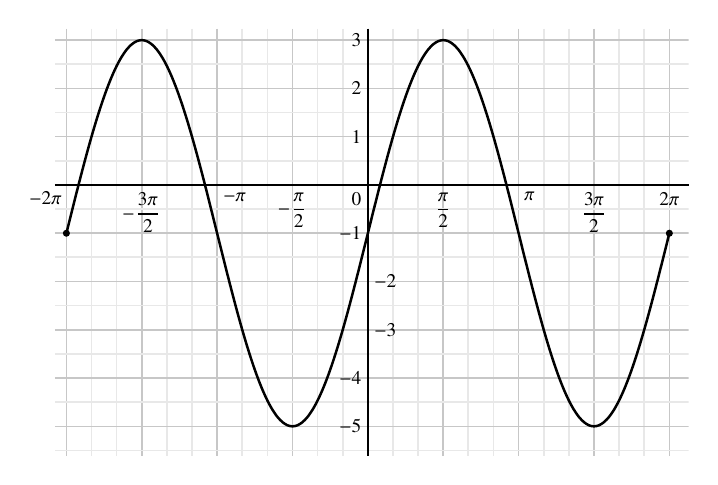
\begin{tikzpicture}[x=0.0127cm,y=-0.0127cm,font=\fontsize{7}{8.4}\selectfont]
\begin{scope}\clip (0,0) rectangle (634,428);
\draw[black!22] (11.4,0)--(11.4,428);
\draw[black!9] (36.5,0)--(36.5,428);
\draw[black!9] (61.7,0)--(61.7,428);
\draw[black!22] (86.8,0)--(86.8,428);
\draw[black!9] (111.9,0)--(111.9,428);
\draw[black!9] (137.1,0)--(137.1,428);
\draw[black!22] (162.2,0)--(162.2,428);
\draw[black!9] (187.3,0)--(187.3,428);
\draw[black!9] (212.5,0)--(212.5,428);
\draw[black!22] (237.6,0)--(237.6,428);
\draw[black!9] (262.7,0)--(262.7,428);
\draw[black!9] (287.9,0)--(287.9,428);
\draw[black!22] (313.0,0)--(313.0,428);
\draw[black!9] (338.1,0)--(338.1,428);
\draw[black!9] (363.3,0)--(363.3,428);
\draw[black!22] (388.4,0)--(388.4,428);
\draw[black!9] (413.5,0)--(413.5,428);
\draw[black!9] (438.7,0)--(438.7,428);
\draw[black!22] (463.8,0)--(463.8,428);
\draw[black!9] (488.9,0)--(488.9,428);
\draw[black!9] (514.1,0)--(514.1,428);
\draw[black!22] (539.2,0)--(539.2,428);
\draw[black!9] (564.3,0)--(564.3,428);
\draw[black!9] (589.5,0)--(589.5,428);
\draw[black!22] (614.6,0)--(614.6,428);
\draw[black!9] (0,422.1)--(634,422.1);
\draw[black!22] (0,398.0)--(634,398.0);
\draw[black!9] (0,373.9)--(634,373.9);
\draw[black!22] (0,349.7)--(634,349.7);
\draw[black!9] (0,325.5)--(634,325.5);
\draw[black!22] (0,301.4)--(634,301.4);
\draw[black!9] (0,277.2)--(634,277.2);
\draw[black!22] (0,253.1)--(634,253.1);
\draw[black!9] (0,228.9)--(634,228.9);
\draw[black!22] (0,204.8)--(634,204.8);
\draw[black!9] (0,180.7)--(634,180.7);
\draw[black!22] (0,156.5)--(634,156.5);
\draw[black!9] (0,132.3)--(634,132.3);
\draw[black!22] (0,108.2)--(634,108.2);
\draw[black!9] (0,84.1)--(634,84.1);
\draw[black!22] (0,59.9)--(634,59.9);
\draw[black!9] (0,35.8)--(634,35.8);
\draw[black!22] (0,11.6)--(634,11.6);
\end{scope}
\draw (0,156.5)--(634,156.5); \draw (313,0)--(313,428);
% y = 4 sin x - 1 on the question domain -2pi..2pi only: px = 313 + 48.0x, py = 156.5 - 48.3y
\draw[line width=0.9pt] plot[smooth,samples=121,domain=-6.2832:6.2832] ({313+48.0*\x},{156.5-48.3*(4*sin(\x r)-1)});
\fill (11.4,204.8) circle[radius=0.045cm]; \fill (614.6,204.8) circle[radius=0.045cm];
\node[inner sep=0.6pt,anchor=north east] at (9,161) {$-2\pi$};
\node[inner sep=0.6pt,anchor=north] at (86.8,162) {$-\dfrac{3\pi}{2}$};
\node[inner sep=0.6pt,anchor=north west] at (166,161) {$-\pi$};
\node[inner sep=0.6pt,anchor=north] at (237.6,162) {$-\dfrac{\pi}{2}$};
\node[inner sep=0.6pt,anchor=north] at (388.4,162) {$\dfrac{\pi}{2}$};
\node[inner sep=0.6pt,anchor=north west] at (467,161) {$\pi$};
\node[inner sep=0.6pt,anchor=north] at (539.2,162) {$\dfrac{3\pi}{2}$};
\node[inner sep=0.6pt,anchor=north] at (614.6,162) {$2\pi$};
\node[inner sep=0.6pt,anchor=north east] at (309,162) {$0$};
\node[inner sep=0.6pt,anchor=west] at (317,253.1) {$-2$};
\node[inner sep=0.6pt,anchor=east] at (309,11.6) {$3$};
\node[inner sep=0.6pt,anchor=east] at (309,59.9) {$2$};
\node[inner sep=0.6pt,anchor=east] at (309,108.2) {$1$};
\node[inner sep=0.6pt,anchor=east] at (309,204.8) {$-1$};
\node[inner sep=0.6pt,anchor=west] at (317,301.4) {$-3$};
\node[inner sep=0.6pt,anchor=east] at (309,349.7) {$-4$};
\node[inner sep=0.6pt,anchor=east] at (309,398.0) {$-5$};\end{tikzpicture}
\end{document}
